\documentclass[12pt,titlepage,german,a4]{article}

\usepackage{graphicx}

\begin{document}
    \title{\bf Miniprojekt: Minimax-Maschine \\ Pflichtenheft}
    \date{Hardware Projekt 2017 \\ 03. Januar 2017}
    \author{Maximilian Lumpe, Niklas Blume, Jan Feuchter, Phu Bac Duong}
    \maketitle

    \tableofcontents

    \newpage

    \section{Einleitung}
    In diesem Miniprojekt im Rahmen des Hardware-Praktikums besch{\"a}ftigen wir uns mit der Minimax-Maschine, welche uns grundlegend aus der Vorlesung "Grundlagen der Rechnerarchitektur" bekannt ist. Zur L{\"o}sung der Aufgaben ist es hierbei notwendig, die vorgegebene Grundstruktur der Maschine geeignet zu erweitern, um die Algorithmen zu realisieren.\\Die Vorbereitung auf unser Projekt wird dokumentiert und strukturiert durch das von uns erstellte Pflichtenheft. Das Pflichtenheft wird nur unsere Vorbereitung beinhalten. Die Ergebnisse werden in einer weiteren Dokumentation enthalten sein.

    \section{Aufgabe: Paketanalyse}
    Nach unserem Verst{\"a}ndniss ist das Ziel der Aufgabenstellung das Implementieren des Algorithmus "Paketanalyse" auf der Minimax-Maschine. Dieser Algorithmus wertet die L{\"a}nge des Nutzdatenteils der Datenpakete aus dem Speicher der Maschine aus.\\Jedes Paket besteht aus einem Header mit 80 Bits, gefolgt von dem Datenteil mit variabler L{\"a}nge. Ein Paket beginnt mit dem festgelegten Bitmuster 1110. Der Header enth{\"a}lt eine 2 Bytes lange Kanalnummer, die bei der Bitstelle 32. beginnt. Zu einem Kanal geh{\"o}ren mehrere Datenpakete mit einer eindeutigen Kanalnummer. Die Anzahl der Bits, die in den Speicher geladen werden, wird als bekannt vorausgesetzt und wird in ein entsprechendes Register vorgeladen.\\Nun soll der "Paketanalyse"-Algorithmus eine Tabelle, die Kanalnummern und zugeh{\"o}rige Datenl{\"a}ngen (in Bits) enth{\"a}lt, anlegen. Haben mehrere Paket dieselbe Kanalnummer, so werden die L{\"a}ngen des Nutzdatenteils zusammengef{\"u}gt. Die Tabelle soll ab einer beliebigen Speicheradresse au{\ss}erhalb des Paketfeldbereichs im Hauptspeicher der Maschine abgelegt werden.\\Diese Aufgabenstellung soll mit dem gegebenen Minimax-Simulator simuliert und getestet werden. Die Maschine kann durch vorgegebene Bauteile erweitert werden, was sich jedoch auf die Bewertung auswirkt. Der Algorithmus wird in Form der Steuertabelle implementiert und soll au{\ss}erdem als Flussdiagramm abgegeben werden.

    \newpage

    \section{Ist-Analyse der Basismaschine}
    Die Minimax-Maschine ist ein minimales Rechensystem welches im Wesentlichen aus einigen Registern (Basis ACCU, PC, IR, MDR, MAR) und einer arithmetisch-logischen Einheit (ALU), welche den Datenpfad bilden, und einem Hauptspeicher (HS) besteht. Jeder Register hat als Eingang mindesten die ALU und zus{\"a}tzlich einen Eingang, der den Schreibzugriff regelt. Der Befehlsablauf des Systems wird {\"u}ber ein Mikroprogramm festgelegt.\\
    F{\"u}r das Projekt kann die Architektur der Minimax-Maschine um zuss{\"a}tzliche Register bzw. Sign Extension Units erweitert werden.
    \begin{itemize}
        \item Die Basismaschine:
        \begin{enumerate}
            \item ACCU: Abk{\"u}rzung f{\"u}r “Accumulator“ ein Zwischenspeicher, um mit MDR Operationen durchf{\"u}hren zu k{\"o}nnen.
            \item PC: Abk{\"u}rzung f{\"u}r “program counter“, enth{\"a}lt den Programmz{\"a}hler, welcher den n{\"a}chsten Befehl beeinflusst.
            \item IR: Abk{\"u}rzung f{\"u}r “instruction register“, enth{\"a}lt Opcode(8 Bit) und Adressteil(24 bit).
            \item MDR: Abk{\"u}rzung f{\"u}r “memory data register“, enth{\"a}lt je nach Einstellung des Multiplexers textttMDR.Sel, verschiede Daten entweder aus Hauptspecher oder aus der ALU.
            \item MAR: Abk{\"u}rzung f{\"u}r “memory adress register“, enth{\"a}lt die Speicheradresse an der ausdem Hauptspeicher Daten geladen oder geschrieben werde sollen.
            \item HS: Abk{\"u}rzung f{\"u}r “Hauptspeicher“, er wird mit 24-Bit durch MAR adressiert und gibt eine 32-Bit Zahl zur{\"u}ck. Auf die selbe Art funktioniert schreiben einer 32-Bit Zahl nat{\"u}rlich auch.
        \end{enumerate}
        \item ALU-Operationen der Basismaschine:
        \begin{enumerate}
            \item ADD: Addiert ALU-Eingang A und ALU-Eingang B
            \item SUB.B: Subtrahiert ALU-Eingang A von ALU-Eingang B
            \item TRANS.A: Schaltet den ALU-Eingang A durch
            \item TRANS.B: Schaltet den ALU-Eingang B durch
        \end{enumerate}
    \end{itemize}
    Die m{\"o}glichen Operationen auf die in der ALU implementieren Operationen sind beschr{\"a}nkt (Basis:  ADD, SUB, TRANS.A, TRANS.B ) . Die ALU kann aber mit zus{\"a}tzliche Operationen , wie z.B dem DIV-Befehl oder dem AND-Befehl, erg{\"a}nzt werden.
    Um eine Operation auszuf{\"u}hren m{\"u}ssen {\"u}ber die Multiplexer ALUSel.A und AluSel.B zwei
    Operanden ausgew{\"a}hlt werden und der ALU muss {\"u}ber die ALU Ctrl-Leitung der Code
    f{\"u}r die Operation {\"u}bergeben werden. An den Multiplexern liegen sowohl Konstanten als
    auch die Register an, welche zur ALU durchgeschaltet werden k{\"o}nnen. Das Ergebnis der
    Operation kann entweder in einem Register ({\"u}ber MDR) oder im HS (Adresse im Register
    MAR) gespeichert werden. Zus{\"a}tzlich k{\"o}nnen Flags (Basis nur ein Flag ALU RESULT ==
    0) gesetzt werden, welche zur{\"u}ck zur Control Unit (CU) geleitet werden um z. B. bedingte
    Spr{\"u}nge auszuf{\"u}hren. \\
    Die uns vorliegende Minimax-Maschine arbeitet mit 32-Bit und speichert Werte mit
    32-Bit in den Registern und im HS. Alle ALU-Operationen werden folglich mit 32-Bit ausgef{\"u}hrt. Dies stellt sich jedoch f{\"u}r unser Aufgabe als Hindernis, da wir die Daten
    bitweise untersuchen m{\"u}ssen, Daten aus dem HS und den Registern jedoch nur als 32-Bit
    Zahlen auslesen k{\"o}nnen und nicht als einzelne Bits.\\
    Folglich wird die Basismaschine um einige Konstanten, Operationen und Register erweitert
    werden m{\"u}ssen, welche im “Implementierungskonzept“ n{\"a}her aufgef{\"u}hrt sind.

    \section{Beschreibung des Implementierungskonzeptes}
    Bei der Implementierung der Paketanalyse muss zwischen mehreren Teilschritten unterschieden werden. Zun{\"a}chst wird nach dem Startbitmuster des ersten Paketes gesucht (1). Ist ein Paket identifiziert, k{\"o}nnen die ersten 32 bits (dies entspricht einer Speicherzelle) {\"u}bersprungen werden (2). Somit beginnt mit der zweiten Speicherzelle die Kanalnummer des Paketes, diese wird extrahiert und abgespeichert (3). Nach 32 weiteren Bits kommt nun der Datenteil, welcher Bit f{\"u}r Bit ausgelesen wird, w{\"a}hrend gleichzeitig ein z{\"a}hlregister inkrementiert wird (4). W{\"a}hrend dieses Vorgangs wird permanent {\"u}berpr{\"u}ft, ob ein neues Startbitmuster vorliegt, sodass ein neues Paket anf{\"a}ngt (5). Ist dies der Fall, wird das Z{\"a}hlregister auf den momentanen Wert f{\"u}r die Kanalnummer addiert. Die Kanalnummer dient dabei als Offset f{\"u}r die Speicherzelle (6).

    \subsection{Identifizierung des Startbitmusters}
    Da f{\"u}r das Startbitmuster nur die vier niedrigwertigsten Bits untersucht werden, m{\"u}ssen zun{\"a}chst f{\"u}r einen Vergleich die restlichen ausgeblendet werden. Dies erfolgt durch eine bitwise-and verkn{\"u}pfung mit Nullen. Anschließend wird das Ergebnis mit dem Startbitmuster verglichen. Sind sie nicht identisch, wird die Speicherzelle geshiftet. Dies wird solange wiederholt, bis das Ergebnis identisch ist, dann wird mit Schritt 2 fortgefahren.

    \subsection{Kanalnummer extrahieren}
    In der ersten Speicherzelle stehen nun die 4 bits des Startmusters, sowie 28 bits die {\"u}bersprungen werden. Also enth{\"a}lt die erste Speicherzelle keine weiteren Informationen, sodass mit der n{\"a}chsten Speicherzelle fortgefahren wird. Nun m{\"u}ssen die ersten 16 bits, die die Kanalnummer beinhalten, extrahiert werden. Hierf{\"u}r sorgt wieder die bitwise-and Verkn{\"u}pfung der restlichen Bits mit Nullen. Die Kanalnummer muss f{\"u}r die sp{\"a}tere Nutzung abgespeichert werden.

    \subsection{Datenbits z{\"a}hlen}
    Auch die zweite Speicherzelle enth{\"a}lt nun keine Informationen mehr. Da in der dritten Speicherzelle noch 16 bits sind, die nicht zum Datenteil geh{\"o}ren, werden im ersten Durchlauf nur 16 auf das Z{\"a}hlregister f{\"u}r die L{\"a}nge des Datenteils addiert. F{\"u}r jeden weiteren Schleifendurchlauf werden dann 32 addiert.

    \subsection{Auf neues Startbitmuster {\"u}berpr{\"u}fen}
    W{\"a}hrend die Datenbit nach und nach durch shiften gez{\"a}hlt werden, wird permanent auch der Test aus (1). durchgef{\"u}hrt. Sobald das Startbitmuster erkannt ist, bricht die Schleife aus (3) ab und es folgt Schritt (5).

    \subsection{Z{\"a}hlregister zur Tabelle hinzuf{\"u}gen}
    Um die Tabelle zur Speicherung der L{\"a}ngen von den eigentlichen Daten zu trennen, darf diese erst in einer Speicherzelle nach der maximalen Datenl{\"a}nge beginnen. Die Adresse der ersten Speicherzelle f{\"u}r die Adresse soll dabei in einem Register gespeichert sein. Nun wird die Kanalnummer auf dieses Register addiert, um die Speicherzelle f{\"u}r eine bestimmte Kanalnummer zu erhalten. Damit hat die Kanalnummer 0 die erste Speicherzelle der Tabelle, die Kanalnummer 1 die zweite, usw. . Auf den Inhalt dieser Speicherzelle wird dann der Inhalt des Z{\"a}hlregisters addiert. Anschlie{\ss}end werden die tempor{\"a}ren Register zur{\"u}ckgesetzt und der Algorithmus beginnt erneut mit Schritt (2).



    \section{Angestrebte Projektergebnisse}
        \begin{itemize}
			\item Ein Pflichtenheft, in dem wir unsere Vor{\"u}berlegungen festhalten.
			\item Eine vollst{\"a}ndige und funktionsf{\"a}hige L{\"o}sung mit allen Testdateien.
			\item Einen Schaltplan, bei dem wir die gegebene Minimax - Maschine um die notwendigen Elemente erweitert haben.
			\item Eine vollst{\"a}ndige Dokumentation, mit der wir unseren Algortihmus und unsere implementierte L{\"o}sung beschreiben und erl{\"a}utern.
        \end{itemize}

	\section{Arbeitsaufteilung}
		\begin{itemize}
			\item Maximilian Lumpe: Einleitung und Aufgabenstellung
			\item Phu Bac Duoung: Ist-Analyse der Basismaschine
			\item Jan Feuchter: Beschreibung des Implementierungskonzeptes
			\item Niklas Blume: Angestrebte Projektergebnisse und Anhang
		\end{itemize}


    \section{Anhang: Flussdiagramme geplanter Mikroprogramme}

	\subsection{Kompletter Algorithmus}

	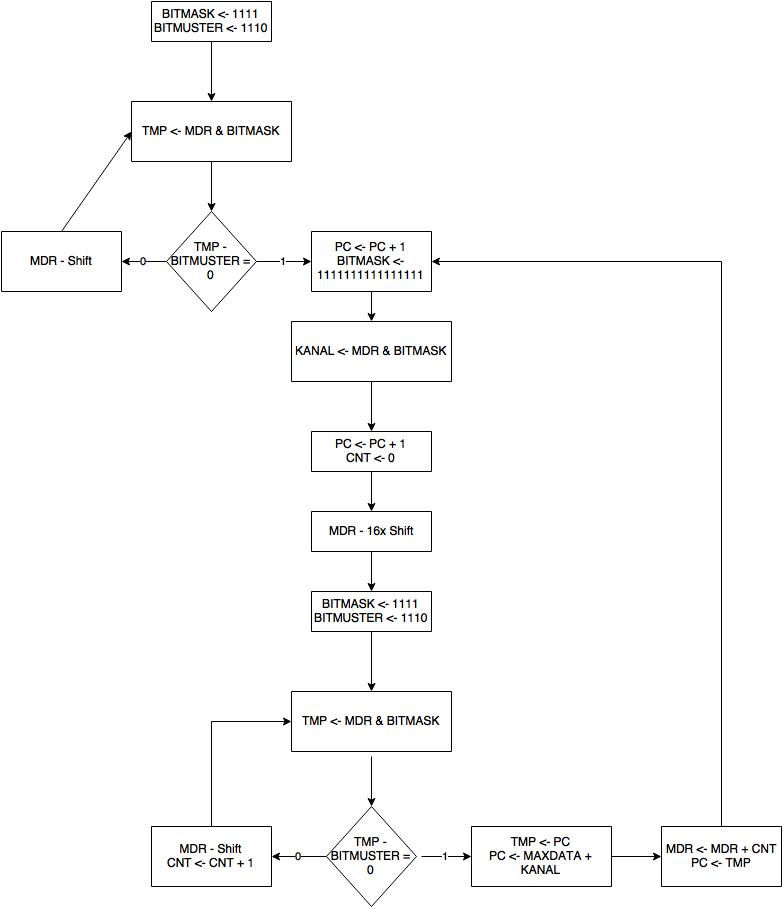
\includegraphics[width=13cm]{algoComplete.png}


	\newpage
    \section{Anhang: Verwendete Hilfsmittel}
	\begin{itemize}
		\item Vorlesung: Grundlagen der Rechnerarchitektur
		\item Umdruck Paketanalyse 2016/17
		\item Minimax - Simulator
		\item GitHub zur Versionskontrolle und Organisation
		\item \string[\url{https://www.draw.io}] zur Erstellung der Flussdiagramme
	\end{itemize}


\end{document}
